\subsection*{Journey to Cornelia}
"Even the moon'd tire of waitin' around for your ass!"\\
\indent-- Cid 
\begin{center} 
	\tcbox[left=0pt,top=0pt,right=0pt,bottom=0pt, boxsep=0pt, colframe=accent, sharp corners]{
		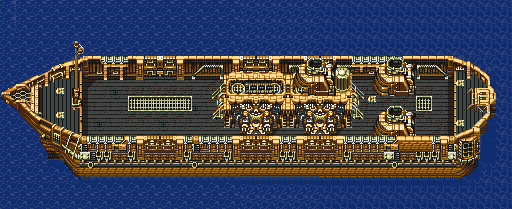
\includegraphics[width=0.98\columnwidth]{./art/maps/ship2.png} 
	}
\end{center}
The adventure starts on a small transport ship named "Tiny Bronco", which is on its way to deliver cargo to the city of Cornelia.
The captain has agreed to let the party board the ship for a small fee.
The ship's crew consists of only 3 members: Biggs, Wedge and Captain Cid.
The two sailors are wearing light blue bandannas and shorts as well as orange shirts with black stripes.
Both are very young and inexperienced, but generally friendly towards the party.
The same cannot be said of the older captain, who retreats to his cabin and prefers to be left alone.

\subsubsection*{Daytime}  
"I don't look like it, but I'm a coward at heart."\\
\indent-- Wedge \\\\
If the adventurers are not familiar beforehand, they should introduce each other first after which they are free to explore the ship.
They can also talk to the sailors who are happy to kill time during the journey.
Biggs and Wedge tell them about recent pirate attacks on sea, which seem to have increased recently.
Furthermore, they may also tell the party about Cornelia, as they have heard that the princess has disappeared.
The party might also ask about Cid, in which case the sailors tell them about his past as a former soldier.
As it begins getting dark outside, the crew retreats to their cabins.
When the adventurers prepare to finish the day as well, they suddenly hear loud noises surrounding the ship.
They quickly realize that several pirates have boarded the Tiny Bronco!

\subsubsection*{Battle on the Tiny Bronco}  
Place roughly one pirate on the ship per party member and spread them around the deck as you see fit.
Meanwhile, the ship's crew is out of sight, fighting other pirates who have entered the ship below deck.
If things end up looking bad for the party during this battle, Biggs and Wedge may come outside to help them.
Their combat details are shown below and are the same as for the pirates.
After defeating the enemies, remember to award the party with the dropped Gil for each slain pirate.
After the battle, the crew comes together with the party and Cid thanks them for their help.
He explains that this is not the first time they have been raided by these pirates, who are part of Captain Bikke's crew.
The party may now go to sleep below deck to fully recover their HP and MP.
Shortly after they wake up in the morning, the ship arrives at Cornelia Port. 
Once there, the crew begins unloading the goods and parts ways with the party.
\vspace{0.5cm}
\monster{Pirate / Biggs / Wedge}{1}{
\includegraphics[width=0.16\textwidth]{./art/monsters/pirate.png}}
{
	HP: & \hfill 8 & MP: & \hfill 0\\
	STR: & \hfill 1 & DEF: & \hfill 0 \\
	MAG: & \hfill 0 & RES: & \hfill 0 \\
	AGI: & \hfill 3 & Size: & \hfill M\\
}
{
	\textbf{Scimitar}: 1d DMG \hfill \textbf{Drops:} 150 Gil 
}
\vspace{0.8cm}
\subsection*{Cornelia Port}
Cornelia Port is small and accommodates only a handful of cargo ships like the Tiny Bronco.
The sailors at the port are unloading boxes from the ships, either to store them in warehouses or carry them directly to Cornelia.
After getting off the ship, the party can ask around to find the way to Cornelia.
The sailors warn to be careful on the way, as the castle guards are not patrolling the route anymore.
Cornelia is not far from the port and the path mostly leads through fields and grassland.
 
%\begin{center} 
\vfill
	\tcbox[left=0pt,top=0pt,right=0pt,bottom=0pt, boxsep=0pt, colframe=accent, sharp corners]{
		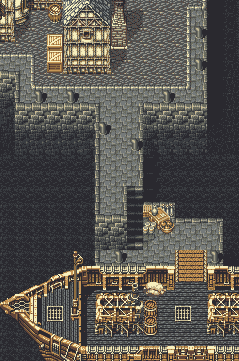
\includegraphics[width=0.97\columnwidth]{./art/maps/port.png} 
	}
%\end{center}

\subsubsection*{Dyce}
"By the by, you need anything? Take a look at my wares! You might just be surprised at what you find..."\\
\indent-- Dyce \\\\
The party can meet a travelling merchant named \textbf{Dyce} at the port.
Dyce is a well built, tall man, bald with beard and wears a dark outfit.
He also has a \hyperlink{chocobo}{Chocobo} at his side that he travels on.
He gives the party information on the troubles in Cornelia, as he has heard rumors about the princess being abducted.
He also sells Potions for 125 Gil each, but he has more inventory which the party cannot afford at this point.
Dyce is a traveller, so there the party will likely meet him again in the future.
His prices are usually be higher compared to regular stores.

\subsubsection*{Battle at Cornelia Port}  
"You must have cannonballs of steel to challenge me!"

-- Bikke \\\\
When talking to Dyce or other sailors, the party finds out that the port is often raided by pirates recently.
Usually, the port is protected by Cornelia's guards, but since the disappearance of the princess, the king has recalled all troops to the castle.
The pirates always attack at night and if the party waits around the port until after dark on any day, they will witness a raid.
As the party knows about their plan, they can try to take defensive measures such as setting up an ambush or traps beforehand.
The attack commences with a large pirate ship docking the port and several pirates storming out to steal pillage the warehouses and other ships.
The pirates are, once again, Captain Bikke's crew, but this time Bikke himself is present as well.
In the ensuing fight, Bikke stays in the back lines and immediately retreats to his ship once he receives any damage. 
There are also some of his men beside him, again roughly one for each party member.
As Bikke likely runs away from this battle, the party may meet him again in the future.
After successfully scaring off the pirates, the sailors at the port are very thankful to the party and offer them free food accommodation for the night.
\vfill
\monster{Bikke}{2}{
\includegraphics[width=0.15\textwidth]{./art/monsters/pirate2.png}}
{
 PV: & \hfill 30 & PM: & \hfill 25\\
 FUE: & \hfill 1 & DEF: & \hfill 2 \\
 MAG: & \hfill 1 & RES: & \hfill 2 \\
 AGI: & \hfill 2 & Tamaño: & \hfill M\\
}
{
 \textbf{Cimitarra}: 1d de daño \mspell{Electro}{4}{0t}{Único}{3u}{Infliges 2d de daño \hyperlink{type}{Eléctrico} al objetivo}{\lightning} \mtech{Arenga}{5}{0t}{Único}{3u}{El objetivo recibe \hyperlink{status}{aumFUE} por 1 turno.}{\enstr} }

\clearpage